\graphicspath{{content/chapters/7_evaluation/figures/}}
\chapter{Evaluation}
\label{chp:evaluation}

This chapter presents a comprehensive evaluation of the implemented speech enhancement system, assessing both classical and deep learning approaches across several dimensions. The evaluation is divided into three key parts. First, the impact of dataset handling strategies is examined, comparing how the different dataset methods affect training efficiency and performance. Second, the effectiveness of Out-of-Memory (OOM) mitigation techniques is validated to ensure that memory-saving strategies do not degrade model quality. Finally, the core focus of this chapter is a comparative analysis of model architectures, benchmarking five machine learning models against three classical denoising methods. Each section includes detailed quantitative assessments using respective metrics. Results are presented using clear, tabulated formats for ease of interpretation and cross-comparison.

\section{Dataset Performance}
\label{sec:dataset_performance}

This section examines the performance of the three dataset handling strategies: Static Bucketing, Dynamic Bucketing, and Padding-Truncation Output-Truncation (PTO). The goal is to assess how these strategies affect the overall efficiency of the training process, particularly in terms of dataset loading times, runtime overhead during training, and their influence on model performance. Each strategy was tested using the same model architecture, the Contextual Encoder-Decoder (CED), chosen for its simplicity and effectiveness in the spectrogram domain. Under two conditions:

\begin{itemize}
    \item \textbf{Cold Run (Uncached):} In this scenario, all dataset operations are executed from scratch. Static and Dynamic Bucketing compute bucket assignments (with Dynamic Bucketing also requiring K-Means clustering), while PTO calculates and stores the original waveform lengths. This setup simulates a first-time deployment or training on a fresh system.
    
    \item \textbf{Warm Run (Cached):} This run utilizes cached data generated during the cold run, significantly reducing load and preprocessing time. For Static and Dynamic Bucketing, bucket mappings and K-Means centers are reloaded. For PTO, the previously computed original sequence lengths are retrieved.
\end{itemize}

The configuration used for all CED runs is shown in Figure~\ref{fig:dataset_config}, with the only varying parameter being the \texttt{PAD\_METHOD}.

\begin{figure}[H]
    \centering
    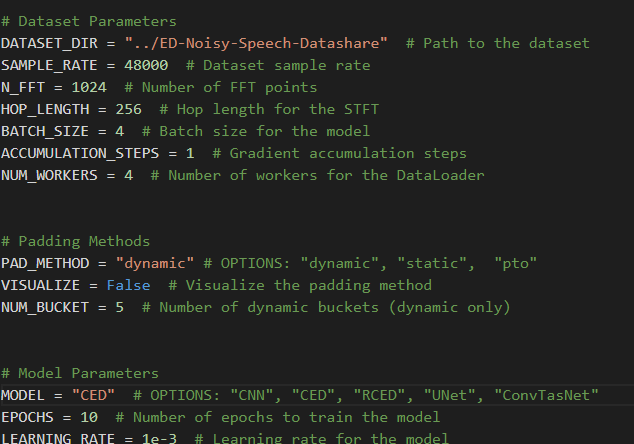
\includegraphics[width=0.8\textwidth]{dataset_config.png}
    \caption{\label{fig:dataset_config} Configuration of the CED model used for dataset performance evaluation.}
\end{figure}

Both uncached and cached runs were executed, and the relevant timing metrics were collected from the output logs, as shown in Table~\ref{tab:dataset_loading_times}.

\vspace{1em}
\begin{table}[H]
\centering
\caption{Dataset Training Overheads}
\label{tab:dataset_loading_times}
\begin{tabular}{|l|c|c|c|}
\hline
\textbf{Dataset} & \textbf{Uncached} & \textbf{Cached} & \textbf{Truncation Overhead} \\
\hline
Static Bucketing  & 296.85 s  & 0.83 s   & N/A    \\
Dynamic Bucketing & 581.57 s& 0.83 s  & N/A    \\
PTO               & 288.47 s & 0.79 s  & 68.62 s  \\
\hline
\end{tabular}
\end{table}

The results in Table~\ref{tab:dataset_loading_times} reveal key insights into the efficiency of each dataset handling strategy. In the uncached condition, both Static Bucketing and PTO exhibit similar loading times, as each only requires a single pass through the dataset. Either to assign buckets or compute original waveform lengths. Dynamic Bucketing, however, incurs nearly double the loading time due to the additional K-Means clustering step, which requires a second pass to calculate cluster centers for optimal bucket assignment. This overhead is particularly pronounced in the uncached scenario, where the dataset must be fully loaded and processed from scratch.

In contrast, the cached runs significantly reduce loading times across all methods. Once the dataset metadata has been computed and stored, subsequent runs simply reload the cached mappings or original lengths, avoiding repeated preprocessing. PTO achieves the fastest cached time, as retrieving a list of original lengths is marginally quicker than reloading bucket assignments or cluster centers. However, a key distinction of PTO is its requirement for per-epoch output truncation during training. While this truncation overhead is relatively minor compared to the total training duration (typically on the order of hours). It can accumulate significantly across large datasets or extended training schedules. This trade-off must be carefully considered when assessing PTO's suitability for time-sensitive or resource-constrained training environments.

To evaluate the impact of dataset handling strategies on model learning, each method was tested using the best-performing checkpoint from its respective training run. Since the differences in performance between cached and uncached conditions were found to be trivial, the results reported in Table~\ref{tab:dataset_performance} reflect the mean values across runs, with corresponding margins of error. This provides a clearer picture of any underlying variation while confirming the consistency of results.

\vspace{1em}
\begin{table}[H]
\centering
\caption{Dataset Handling Strategies Training Metrics}
\label{tab:dataset_performance}
\begin{tabular}{|l|c|c|c|}
\hline
\textbf{Dataset} & \textbf{Train Loss} & \textbf{Val Loss} & \textbf{Val SNR} \\
\hline
Static Bucketing  & \(0.1805 \pm 0.0013\)  & \(0.1787 \pm 0.0020\)  & \(0.54 \pm 0.045\) dB \\
Dynamic Bucketing & \(0.1779 \pm 0.0004\)  & \(0.1850 \pm 0.0063\)  & \(0.56 \pm 0.010\) dB \\
PTO               & \(0.1414 \pm 0.0019\)  & \(0.1458 \pm 0.0033\)  & \(0.53 \pm 0.050\) dB \\
\hline
\end{tabular}
\end{table}

The results in Table~\ref{tab:dataset_performance} show that while all three dataset handling strategies yield reasonable and consistent validation SNR values, there are notable differences in training and validation loss. In particular, the PTO method achieves lower training and validation loss compared to both Static and Dynamic Bucketing. This suggests that PTO facilitates more learning under the current loss formulation.

However, despite its lower loss, PTO does not yield a corresponding improvement in validation SNR. The SNR values across all methods remain within a narrow range, indicating that the perceptual or energy-based denoising quality is comparable. The improved loss values in PTO may be partly influenced by its output truncation mechanism. This evaluates only the central, non-padded regions of the spectrogram. Potentially leading to more favorable loss estimates even if the actual perceptual improvement is marginal.

Considering the trade-offs between implementation complexity, runtime overhead, and generality. Dynamic Bucketing remains the most balanced choice. It handles variable-length inputs with optimal bukceting and minimal padding. Avoids the per-epoch truncation overhead of PTO and maintains reliable performance across all metrics. As such, Dynamic Bucketing is selected as the preferred dataset handling strategy for all subsequent model evaluations in this project.

\section{OOM Validation}
\label{sec:oom_validation}

While Section~\ref{sec:oom_handling} outlined several techniques to mitigate Out-of-Memory (OOM) errors during training. It is important to demonstrate that these strategies do not compromise model learning. The goal of this section is to validate that memory-saving methods do not lead to information loss or degraded performance. To assess this, the RCED model was used, since the UNet and ConvTasNet could not be trained without OOM-handling techniques. Training was conducted using the dynamic bucketing strategy and compared across three different configurations:

\begin{enumerate}
    \item \textbf{Clean Training (Baseline):} A standard training loop without any OOM-handling logic, using a batch size of 4. This configuration serves as the control, with no memory management mechanisms.
    
    \item \textbf{OOM Handling (Batch 4, Accum 1):} OOM-handling techniques were enabled while maintaining a batch size of 4. These included fixed-point precision (FP16) and garbage collection (GC), allowing for a more memory-efficient training process.
    
    \item \textbf{OOM + Accumulation (Batch 2, Accum 2):} The batch size was reduced to 2, with gradient accumulation set to 2, simulating an effective batch size of 4. All OOM-handling techniques remained enabled. This configuration is designed to reduce memory usage while preserving gradient stability.
\end{enumerate}

Each configuration was trained for the same number of epochs, using identical learning rates and optimizers. Table~\ref{tab:oom_training} summarizes the training and validation performance.

\vspace{1em}
\begin{table}[H]
\centering
\caption{OOM Configurations Training Metrics}
\label{tab:oom_training}
\begin{tabular}{|l|c|c|c|c|}
\hline
\textbf{Train Config} & \textbf{Train Loss} & \textbf{Val Loss} & \textbf{Val SNR} & \textbf{Training Time} \\
\hline
Baseline               & 0.1169 & 0.1185 & 3.20 dB & 4.44 h \\
OOM Handling           & 0.1217 & 0.1255 & 2.74 dB & 3.08 h \\
OOM + Accumulation     & 0.1184 & 0.1263 & 2.95 dB & 3.91 h \\
\hline
\end{tabular}
\end{table}

The results in Table~\ref{tab:oom_training} show that all three training configurations achieve comparable performance in terms of both loss and validation SNR. The baseline configuration, which does not use any OOM-handling mechanisms, achieves the best validation SNR of 3.20 dB. With the differences across configurations being within a 0.5 dB range. Suggesting that the inclusion of OOM-handling strategies does include some degradation of the models training performance. The OOM Handling configurations, use of FP16 and GC could be seen as a trade-off between memory efficiency and model performance. 

Each configuration was further evaluated in the full denoising pipeline. Table~\ref{tab:oom_metrics} presents the performance metrics across key evaluation criteria.

\vspace{1em}
\begin{table}[H]
\centering
\caption{OOM Configurations Denoising Metrics}
\label{tab:oom_metrics}
\begin{tabular}{|l|c|c|c|c|c|}
\hline
\textbf{Train Config} & \textbf{↑SNR} & \textbf{↓MSE} & \textbf{↑PESQ} & \textbf{↑STOI} & \textbf{↓LSD} \\
\hline
Baseline               &  14.2843 & 0.000120 & 2.1096 & 0.8730 & 0.702311 \\
OOM Handling           & 14.7731 & 0.000114 & 2.1791 & 0.8783 & 0.691936 \\
OOM + Accumulation     & 14.8076 & 0.000117 & 2.1008 & 0.8748 & 0.692152 \\
\hline
\end{tabular}
\end{table}

The results in Table~\ref{tab:oom_metrics} reveal that, contrary to initial expectations, the OOM-handling configurations not only maintain performance but slightly outperform the baseline in several key denoising metrics. Both the \textbf{OOM Handling} and \textbf{OOM + Accumulation} setups show improvements in SNR, PESQ, and LSD, suggesting enhanced perceptual quality and spectral fidelity.

Specifically, \textbf{OOM + Accumulation} achieves the highest SNR at 14.81 dB, marginally outperforming both the baseline and the non-accumulated OOM variant. Additionally, the lowest LSD values are observed in the OOM-handled models, indicating that their outputs more closely preserve the spectral characteristics of the clean reference signals. These findings suggest that the use of FP16 precision and memory-aware strategies does not harm. Potentially even improving the model's ability to generalize. 

The marginal gains in PESQ and STOI further support this conclusion. Although the differences are subtle, they point to a stable perceptual consistency across configurations. It is also possible that reduced numerical precision in FP16 introduces a form of implicit regularization, slightly mitigating overfitting and improving generalization performance.

In summary, while the training metrics in Table~\ref{tab:oom_training} showed modest differences across configurations. The downstream denoising evaluation shows no degradation and in some cases minor improvements. These findings fully justify the use of OOM-handling techniques throughout this project. Even if future configurations exhibited performance regressions due to OOM mitigation. Their use would remain essential for enabling the training of memory-intensive models such as \textit{UNet} and \textit{Conv-TasNet}, ensuring a fair architectural comparison across all model types evaluated in this work.

\section{Model Performance}
\label{sec:model_performance}

This section presents the most critical part of the evaluation and the central focus of the project. A comparative assessment of classical methods and five machine learning models for speech enhancement. Unlike earlier evaluations, which focused on dataset handling strategies and OOM mitigation techniques using fixed models to conduct the justification. The main scope of this project is to justify the use of machine learning models for speech enhancement and to evaluate their performance against classical methods.

The evaluation retains the previously established dynamic bucketing and OOM handling strategies but now focuses on how model design impacts training efficiency and denoising performance. The section begins with an analysis of classical denoising methods to establish a meaningful baseline for comparison.

\subsection{Classical Methods}
\label{sec:classical_methods}

The classical methods evaluated include Spectral Subtraction (SS), Wiener Filtering (WF), and the Minimum Mean Square Error - Log Spectral Amplitude estimator (MMSE-LSA), all implemented in a single-channel setting. SS and WF are foundational methods in literature, whilst MMSE-LSA represents a more developed and perceptually motivated approach. Since these methods do not require training, the classical evaluation bypasses training and instead focuses solely on denoising performance using the same pipeline and evaluation metrics as the learning-based models.


\vspace{1em}
\begin{table}[H]
\centering
\caption{Classical Denoised Metrics}
\label{tab:classical_metrics}
\begin{tabular}{|l|c|c|c|c|c|c|}
\hline
\textbf{Method} & \textbf{↑SNR} & \textbf{↓MSE} & \textbf{↑PESQ} & \textbf{↑STOI} & \textbf{↓LSD} & \textbf{Denoise Time} \\
\hline
SS          & 1.5406 & 0.002210 & 1.4574 & 0.8538 & 0.7747 & 01.17 m \\
WF          & -3.3796 & 0.006702 & 1.8721 & 0.8968 & 0.9278 & 01.33 m \\
MMSE-LSA    & -2.3929 & 0.005440 & 2.0671 & 0.8974 & 0.8274 & 01.51 m \\
\hline
\end{tabular}
\end{table}


The results in Table~\ref{tab:classical_metrics} highlight key trade-offs between signal fidelity and perceptual quality. SS achieved the best SNR and MSE, suggesting strong numerical suppression of noise. However, it underperformed in perceptual metrics, likely due to spectral distortion and residual artifacts introduced by aggressive subtraction.

In contrast, WF and MMSE-LSA produced negative SNR values indicating that the residual noise after denoising exceeds the remaining speech energy. This behavior is in a purley energy based metric sense but stems from the design of both methods, which prioritize perceptual quality over strict numerical fidelity. In a sense they tolerate or redistribute residual noise in less perceptually important regions of the speech signal. Resulting in improved PESQ and STOI scores despite poorer SNR outcomes. 

Interestingly, although SNR deteriorates, the MSE values remain comparable to those of SS. This can be attributed to the logarithmic nature of SNR versus the linear nature of MSE. Small differences in error magnitude can result in disproportionately large shifts in SNR. Thus, while the total error remains moderate. Its energy distribution leads to poorer SNR without severely impacting overall error magnitude.

These results align with MMSE-LSA's perceptually motivated design, confirming its effectiveness in preserving speech intelligibility and naturalness. Notably, all classical methods completed denoising in under two minutes, indicating no significant computational cost differences.

\subsection{Training The ML Models}
\label{sec:training_ml_models}

With the classical methods evaluated, the focus now shifts to the machine learning models. Each model defined in the \ref{sec:ml_models} section was trained using the same dataset handling strategies and OOM mitigation techniques previously established. The models followed a consistent training configuration: a batch size of 2, accumulation steps of 4, 25 training epochs, and a learning rate of $1 \times e^{-3}$. The table below summarizes the training performance for each model.

\vspace{1em}
\begin{table}[H]
\centering
\caption{Machine Learning Models Training Metrics}
\label{tab:ml_training}
\begin{tabular}{|l|c|c|c|c|}
\hline
\textbf{Model} & \textbf{Train Loss} & \textbf{Val Loss} & \textbf{Val SNR} & \textbf{Training Time} \\
\hline
CNN         & 0.8813 & 0.8883 & 1.06 dB & 3.22 h \\
CED         & 0.8302 & 0.8334 & 1.10 dB & 5.27 h \\
RCED        & 0.8001 & 0.8071 & 1.11 dB & 7.32 h \\
UNet        & 0.7941 & 0.8003 & 1.12 dB & 14.32 h \\
ConvTasNet  & 0.0764 & 0.0760 & 4.76 dB & 13.09 h \\
\hline
\end{tabular}
\end{table}

The training outcomes summarized in Table~\ref{tab:ml_training} clearly demonstrate a consistent yet incremental improvement across the machine learning models from CNN to UNet, followed by a significant leap in performance with ConvTasNet.  

The CNN model was introduced as a simple baseline to validate the project’s training and evaluation pipeline. Despite its minimal architecture, it delivered solid performance and served as a reference point for more advanced models. The training plot in Figure~\ref{fig:cnn_training_plot} provides a quick visual overview of the model's learning progression. Although a small gap between training and validation loss is observed, which might suggest mild overfitting. The magnitude of this gap (0.007) is negligible, and the model retains good generalization performance, making it a reliable benchmark. A similar trend is observed across the remaining models, with no significant signs of overfitting.

\begin{figure}[H]
    \centering
    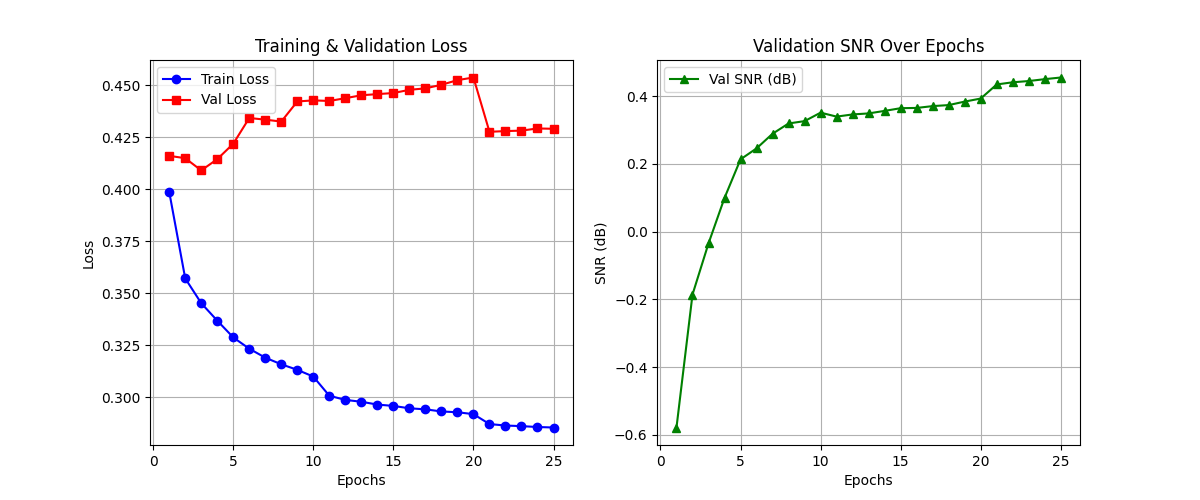
\includegraphics[width=0.8\textwidth]{CNN_plot.png}
    \caption{\label{fig:cnn_training_plot} CNN training plot.}
\end{figure}

The CED model expanded upon the CNN baseline with a fully connected encoder-decoder architecture, yielding modest improvements. Notably, CED demonstrated remarkable training stability, as illustrated in Figure~\ref{fig:ced_training_plot}. The absence of significant fluctuations in the loss curves underscores its effective learning and convergence behavior.

\begin{figure}[H]
    \centering
    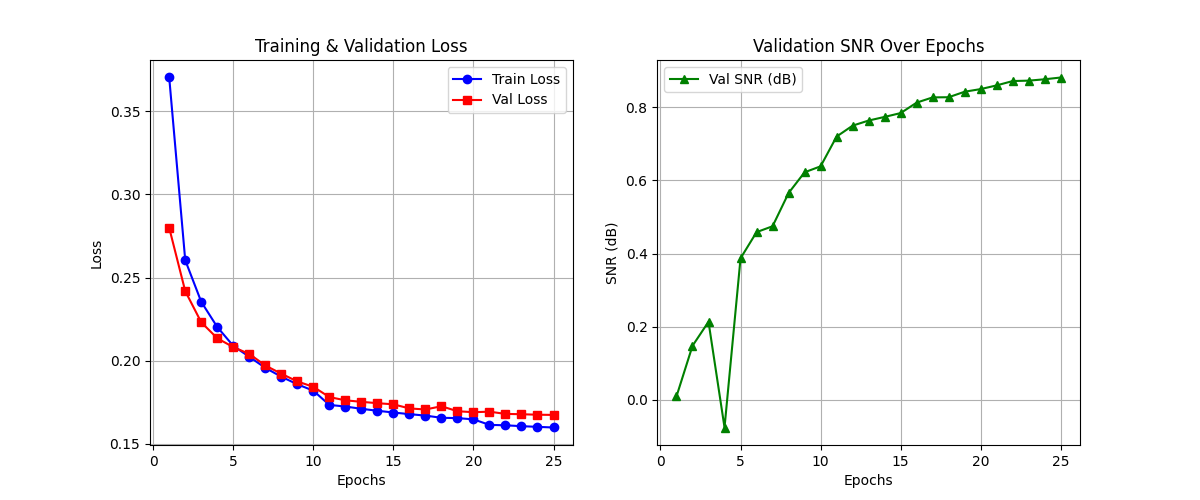
\includegraphics[width=0.8\textwidth]{CED_plot.png}
    \caption{\label{fig:ced_training_plot} CED training plot.}
\end{figure}

The RCED model further improved upon the CED architecture by incorporating residual connections between layers. This enhancement aimed at facilitating better information flow and gradient propagation. The training plot in Figure~\ref{fig:rced_training_plot} still potrays a good learning curve, with slight increase in training time due to the added complexity of the architecture. The fact that RCED already shows improved training metrics over CED, indicated that we will likely see the same trend in the denoising evaluation. Overall confirming \cite{park2017acoustic}’s findings that residual connections can enhance performance in speech enhancement tasks.

\begin{figure}[H]
    \centering
    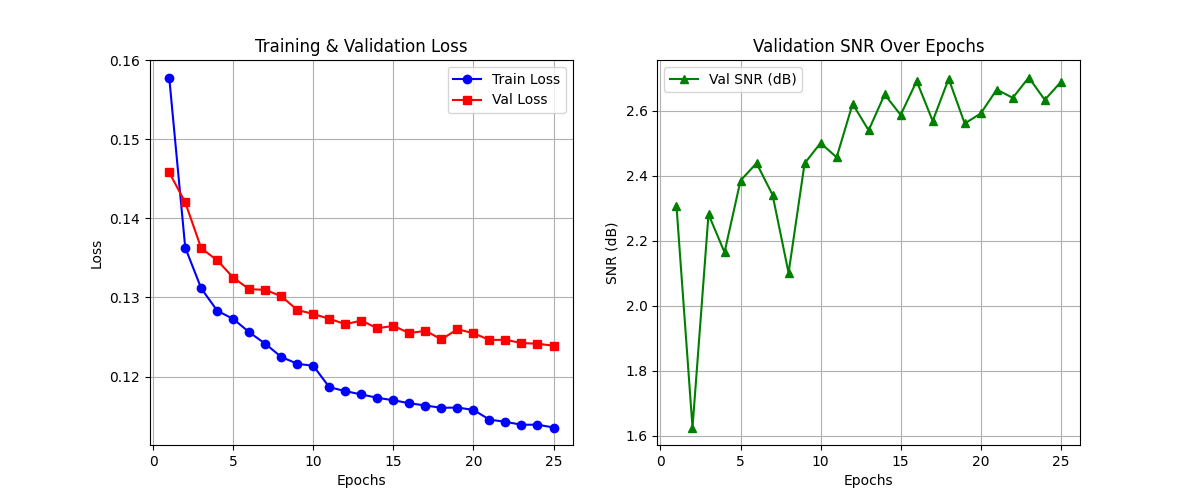
\includegraphics[width=0.8\textwidth]{RCED_plot.png}
    \caption{\label{fig:rced_training_plot} RCED training plot.}
\end{figure}

The UNet was the longets model trained (14.32 h), with almost double the training time of RCED (7.32 h). This increase is naturally attributed from the increaded complexity of the architecture. There are no significant statements to be made about the training plot in Figure~\ref{fig:unet_training_plot}. However, it was expected to show a more pronounced improvement over RCED, given its more complex architecture and doubled training time. It only followed the trend of marginal improvements.

\begin{figure}[H]
    \centering
    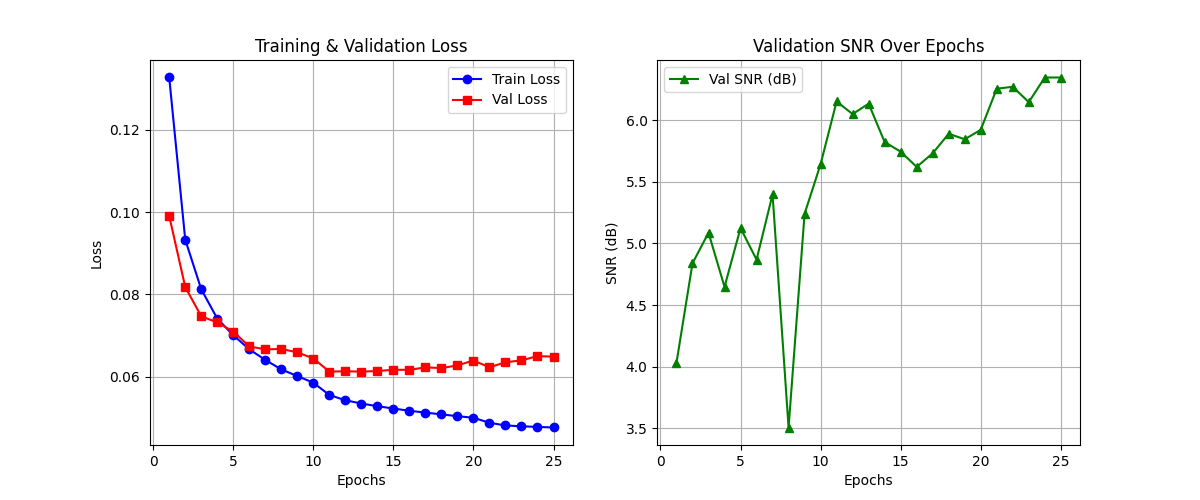
\includegraphics[width=0.8\textwidth]{UNet_plot.png}
    \caption{\label{fig:unet_training_plot} UNet training plot.}
\end{figure}

The most notable result came from ConvTasNet, which showed a significant leap in validation SNR from 1.12 dB (in UNet) to 4.76 dB. The losses didn't illustrate the same drammatic improvement but still gave more substantial improvements. This distinction can also be seen in the training plot in Figure~\ref{fig:convtasnet_training_plot}, as the SNR plot shows signifcant spikes and dips. Indicating that the model is learning to capture complex temporal and spectral patterns in the data. Although evalutaion cannot be solely based on training metrics and require the proper denoising pipeline evlaution along with the metrics. This poses a hopeful outlook for the model's performance in the denoising evaluation and could overcome the limitations of the previous models to make signifcant improvements.

\begin{figure}[H]
    \centering
    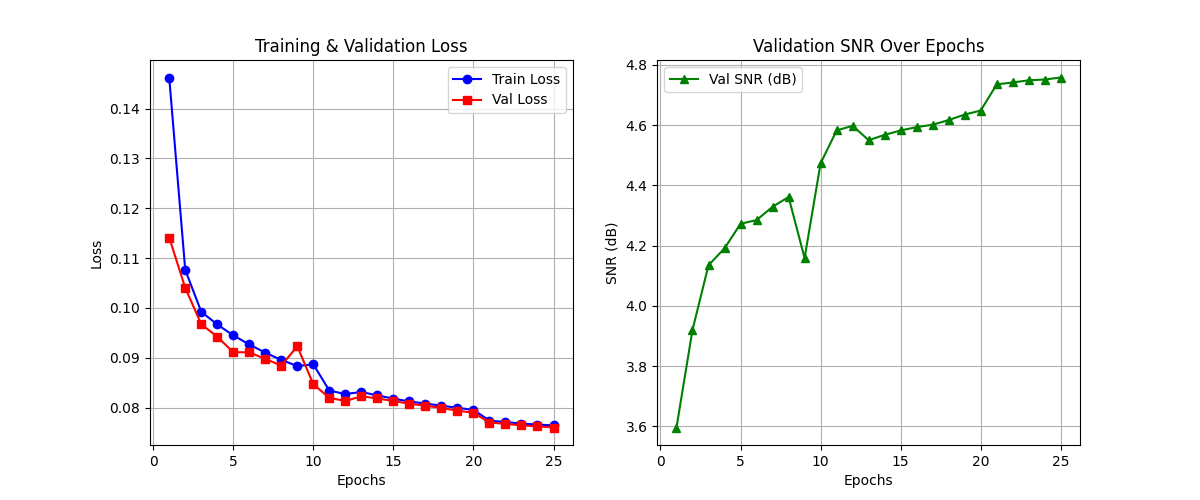
\includegraphics[width=0.8\textwidth]{ConvTasNet_plot.png}
    \caption{\label{fig:convtasnet_training_plot} ConvTasNet training plot.}
\end{figure}

\subsection{Denoising The ML Models}
\label{sec:denoising_ml_models}

Following the training phase, each machine learning model was evaluated using the same denoising pipeline and metrics used for the classical methods. The table below summarizes the performance of all five models across objective and perceptual metrics, as well as their denoising runtime.

\vspace{1em}
\begin{table}[H]
\centering
\caption{Machine Learning Denoising Metrics}
\label{tab:ml_denoise}
\begin{tabular}{|l|c|c|c|c|c|c|}
\hline
\textbf{Model} & \textbf{↑SNR} & \textbf{↓MSE} & \textbf{↑PESQ} & \textbf{↑STOI} & \textbf{↓LSD} & \textbf{Denoise Time} \\
\hline
CNN         & 0.4715  & 0.002340 & 1.1906 & 0.7351 & 0.9639 & 01.28 m \\
CED         & 0.8615  & 0.002138 & 1.1626 & 0.7847 & 0.9210 & 01.24 m \\
RCED        & 0.9655  & 0.002088 & 1.2825 & 0.8115 & 0.9031 & 01.29 m \\
UNet        & 0.9844  & 0.002079 & 1.3273 & 0.7983 & 0.9206 & 01.38 m \\
ConvTasNet  & 17.9050 & 0.000063 & 2.3001 & 0.9001 & 0.6881 & 01.44 m \\
\hline
\end{tabular}
\end{table}
The results in Table~\ref{tab:ml_denoise} show the performance progression across models, reflecting implementation improvements made throughout the project. The baseline CNN model delivers reasonable perceptual quality out-of-the-box but underperforms significantly in terms of SNR. While its MSE remains comparable to that of the CED and RCED models, its SNR is nearly halved. Since SNR and MSE both mathematically represent the difference between clean and denoised signals, this discrepancy suggests that CNN likely retains higher-energy residual noise. Although the total error magnitude (MSE) may be similar, the CNN's denoised output likely introduces noise that disproportionately affects the signal's energy ratio, thus reducing the SNR. This underscores the importance of evaluating both energy-based and perceptual metrics together, as the CNN still maintains moderate PESQ and STOI scores despite its weaker SNR.

The CED and RCED models, both adapted from \cite{park2017acoustic}, were introduced to address limitations observed in the CNN baseline by incorporating fully connected encoder-decoder architectures. CED better suits the structured nature of spectrograms, capturing broader contextual information. Consequently, it achieves a clear improvement in SNR (\textbf{0.86 dB}) compared to CNN (\textbf{0.47 dB}), effectively resolving the earlier energy imbalance issue. RCED enhances this approach by adding residual connections between layers, which help preserve information flow and stabilize gradient propagation during training. This leads to further gains across all metrics, with RCED achieving higher PESQ (\textbf{1.28}) and STOI (\textbf{0.81}) scores than both CNN and CED, along with slight improvements in MSE and SNR.

These outcomes align with the original findings in \cite{park2017acoustic}, where residual connections were shown to improve speech enhancement performance. Despite these gains, both CED and RCED architectures have structural limitations. Using a single bottleneck without feature merging across scales can lead to the loss of fine-grained spectral details during encoding and decoding. While RCED partially mitigates this through residual connections, it lacks the explicit skip connections found in UNet, which help reintegrate high-resolution features during decoding.

The UNet model extends the encoder-decoder structure with these skip connections, enabling the recovery of fine-grained spectral details lost during downsampling and improving the model’s ability to capture both local and global context. UNet continues the incremental gains over previous models. However, as mentioned in Section \ref{sec:training_ml_models}, there is a suboptimal efficiency-performance tradeoff. This may stem from the project's implementation of the architecture or because the scope in which the architecture was applied does not align closely with its core design purpose. Furthermore, none of the models from CNN to UNet surpassed the perceptual quality performance of classical methods such as Wiener Filtering or MMSE-LSA. This raises questions regarding whether the added complexity and training overhead of these models are justified for real-world deployment.

However, the promising results portrayed by ConvTasNet in Section \ref{sec:training_ml_models} were strongly confirmed in the denoising evaluation. ConvTasNet achieved a remarkable results both for numerical and perceptual metrics. The SNR of \textbf{17.90 dB} is more than 18 times higher than the UNet's \textbf{0.98 dB}. Which may seem like an unrealistic leap at first, but is actually a result of the model's design. It perceptual results also improved significantly, with PESQ of \textbf{2.30}, STOI of \textbf{0.90}, and LSD of \textbf{0.69}. 

- Add metrics of pre-trained models to show comparable and realistic results.
- Discuss optimality of ConvTasNet coming from effective porting (possible unlike UNet) of the defined model architecture in time domain to our spectrogram domain.
- State that we could have also possibly saturated the model through the magnitude masking.

\vspace{2em}

- Add a small note that the ConvTasNet model undergoe limited hyperparameter tuning given the constrained environment. But the more optimized paramteres where not significantly different from the initial testing ones and provide x more performance.


\section{Subjective Evaluation}
\label{sec:subjective_evaluation}

